\chapter{Week 6}
\section{ML:Advice for Applying Machine Learning}
\subsection{Deciding what to do next}
Errors in your predictions can be troubleshooted by:
\begin{itemize}
	\item Getting more training examples
	\item Trying smaller sets of values
	\item Trying additional features
	\item Trying polynomial features
	\item Increasing ore decreasing $\lambda$
\end{itemize}
Don't just pick one of these avenues at random. We'll explore diagnostic techniques for choosing one of the above solutions in the following sections.
\section{Evaluating a Hypothesis}
A hypothesis may have low error for the training examples but still be inaccurate (because of overfitting).

With a given dataset of training examples, we can split up the data into two sets: a \textbf{training set} and a \textbf{test set}.

The new procedure using these two sets is then:

\begin{enumerate}
	\item Learn $\Theta$ and minimize $J_{train}(\Theta)$ using the training set.
	\item Compute the test set error $J_{test}(\Theta)$
\end{enumerate}
\subsection{The test set error}
\begin{enumerate}
\item For linear regression
\[J_{test}(\Theta) = \dfrac{1}{2m_{test}} \sum_{i=1}^{m_{test}}(h_\Theta(x^{(i)}_{test}) - y^{(i)}_{test})^2
\]
\item For classification $\sim$ Miscalssification error (aka 0/1 misclassification error):
\end{enumerate}
\begin{equation}
err(h_\Theta(x),y) =
\begin{matrix}
1 & \mbox{if } h_\Theta(x) \geq 0.5\ and\ y = 0\ or\ h_\Theta(x) < 0.5\ and\ y = 1\newline
0 & \mbox otherwise 
\end{matrix}
\end{equation}
This givw us a binary 0 or 1 error result based on a misclassification.

The average test error for the test set is
\[
\text{Test Error} = \dfrac{1}{m_{test}} \sum^{m_{test}}_{i=1} err(h_\Theta(x^{(i)}_{test}), y^{(i)}_{test})
\]
This give us the proportion of the test data that was misclassified.

\section{Model Selection and Training/Validation/Test Sets}
\begin{itemize}
\item Just because a learning algorithm fits a training set well, that does not mean it is a good hypothesis.
\item The error of your hypothesis as measured on the data set with which you trained the parameters will be lower than any other data set.
\end{itemize}

In order to choose the model of your hypothesis, you can test each degree of polynomial and look at the error result.

\subsection{Without the Validation Set (note: this is a bad method - do not use it)}
\begin{enumerate}
\item Optimize the parameters in $\Theta$ using the training set for each polynomial degree.
\item Find the polynomial degree d with the least error using the \textbf{test set}
\item Estimate the generalization error also using the test set with $J_{test}(\Theta^{(d)})$, (d = theta from polynomial with lower error);
\end{enumerate}
In this case, we have trained one variable, d, or the degree of the polynomial, using the test set. This will cause our error value to be greater for any other set of data.
\subsection{Use of the CV set}
To solve this, we can introduce a third set, the \textbf{Cross Validation Set}, to serve as an intermediate set that we can train d with. Then our test set will give us an accurate, non-optimistic error:

One example way to break down our dataset into the three sets is:
\begin{itemize}
\item Training set: 60\%
\item Cross validation set: 20\%
\item Test set: 20\%

\end{itemize}
We can now calculate three separate error values for the three different sets.

\textbf{With the Validation Set (note: this method presumes we do not also use the CV set for regularization)}

\begin{enumerate}
\item Optimize the parameters in $\Theta$ using the training set for each polynomial degree.
\item Find the polynomial degree d with the least error using the cross validation set.
\item Estimate the generalization error using the test set with $J_{test}(\Theta^{(d)})$, (d = theta from polynomial with lower error);
\end{enumerate}

This way, the degree of the polynomial d has not been trained using the test set.

(Mentor note: be aware that using the \textbf{CV set} to select `d' means that we cannot also use it for the validation curve process of setting the lambda value).

\section{Diagnosing Bias vs. Variance}
In this section we examine the relationship between the degree of the polynomial d and the underfitting or overfitting of our hypothesis.
\begin{itemize}
\item We need to distinguish whether \textbf{bias} or \textbf{variance} is the problem contributing to bad predictions.
\item High bias is underfitting and high variance is overfitting. We need to find a golden mean between these two.
\end{itemize}

The training error will tend to \textbf{decrease} as we increase the degree d of the polynomial.

At the same time, the cross validation error will tend to \textbf{decrease} as we increase d up to a point, and then it will \textbf{increase} as d is increased, forming a convex curve
\subsection{High bias (underfitting): }
$J_{train}(\Theta)$ and $J_{CV}(\Theta)$ will be high. Also, $J_{CV}(\Theta) \approx J_{train}(\Theta)$ 
\subsection{High variance (overfitting):}
$J_{train}(\Theta)$ will be low and $J_{CV}(\Theta)$  will be much greater than $J_{train}(\Theta)$

This is represented in the figure \ref{fig:W6_polydeg}
\begin{figure}[ht]
\center
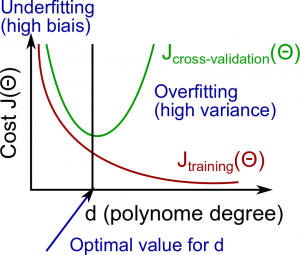
\includegraphics[scale=0.6]{W6_polydeg}
\caption{Polynomial degree}
\label{fig:W6_polydeg}
\end{figure}
\section{Regularization and Bias/Variance}
Instead of looking at the degree d contributing to bias/variance, now we will look at the regularization parameter $\lambda$.

\begin{itemize}
\item Large $\lambda$: High bias (underfitting)
\item Intermediate $\lambda$: just right
\item Small $\lambda$: High variance (overfitting)
\end{itemize}

A large lambda heavily penalizes all the $\Theta$ parameters, which greatly simplifies the line of our resulting function, so causes underfitting.

The relationship of $\lambda$ to the training set and the variance set is as follows:

\begin{itemize}
\item \textbf{Low $\lambda$}: $J_{train}(\Theta)$ is low and $J_{CV}(\Theta)$ is high (high variance/overfitting).
\item \textbf{Intermediate $\lambda$}: $J_{train}(\Theta)$ and $J_{CV}(\Theta)$ are somewhat low and $J_{train}(\Theta) \approx J_{CV}(\Theta)$
\item \textbf{Large $\lambda$}: both $J_{train}(\Theta)$ and $J_{CV}(\Theta)$ will be high (underfitting /high bias)
\end{itemize}

The figure \ref{fig:W6_polydeg2} illustrates the relationship between lambda and the hypothesis:

\begin{figure}[ht]
\center
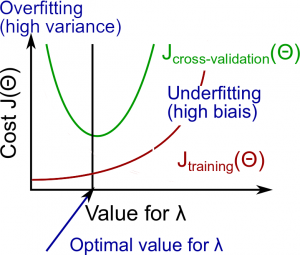
\includegraphics[scale=0.6]{W6_polydeg2}
\caption{relationship between lambda and the hypothesis}
\label{fig:W6_polydeg2}
\end{figure}

In order to choose the model and the regularization $\lambda$, we need:
\begin{enumerate}
\item Create a list of lambdas 

(i.e. $\lambda\in$\{0,0.01,0.02,0.04,0.08,
0.16,0.32,0.64,1.28,2.56,5.12,10.24\});
\item Create a set of models with different degrees or any other variants.
\item Iterate through the $\lambda$'s and for each $\lambda$ go through all the models to learn some $\Theta$.
\item Compute the cross validation error using the learned $\Theta$ (computed with $\lambda$) on the $J_{CV}(\Theta)$ without regularization or $\lambda = 0$.
\item Select the best combo that produces the lowest error on the cross validation set.
\item Using the best combo $\Theta$ and $\lambda$, apply it on $J_{test}(\Theta)$ to see if it has a good generalization of the problem.
\end{enumerate}
\section{Learning Curves}
Training 3 examples will easily have 0 errors because we can always find a quadratic curve that exactly touches 3 points.
\begin{itemize}
\item As the training set gets larger, the error for a quadratic function increases.
\item The error value will plateau out after a certain m, or training set size.
\end{itemize}
\subsection{With high bias}
\textbf{Low training set size}: causes $J_{train}(\Theta)$to be low and $J_{CV}(\Theta)$ to be high.

\textbf{Large training set size}: causes both $J_{train}(\Theta)$ and $J_{CV}(\Theta)$ to be high with $J_{train}(\Theta) \approx J_{CV}(\Theta)$

If a learning algorithm is suffering from \textbf{high bias}, getting more training data \textbf{will not (by itself) help much}.

For high variance, we have the following relationships in terms of the training set size:
\subsection{With high variance}
\textbf{Low training set size}: $J_{train}(\Theta)$ will be low and $J_{CV}(\Theta)$ will be high.

\textbf{Large training set size}: $J_{train}(\Theta)$ increases with training set size and $J_{CV}(\Theta)$ continues to decrease without leveling off. Also, $J_{train}(\Theta)<J_{CV}(\Theta)$ but the difference between them remains significant.

If a learning algorithm is suffering from \textbf{high variance}, getting more training data is \textbf{likely to help}.
\begin{figure}[ht]
     \centering
     \begin{subfigure}[b]{0.47\textwidth}
         \centering
         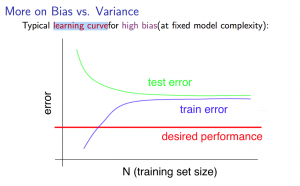
\includegraphics[width=\textwidth]{W6_LC1}
         \caption{More on Bias vs Variance}
         \label{fig:W6_LC1}
     \end{subfigure}
     \hfill
     \begin{subfigure}[b]{0.47\textwidth}
         \centering
         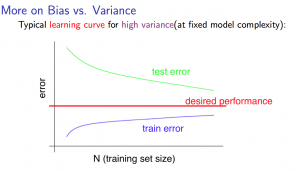
\includegraphics[width=\textwidth]{W6_LC2}
         \caption{More on Variance vs Bias}
         \label{fig:W6_LC2}
     \end{subfigure}
     \caption{Learning Curves}
     \label{fig:W6_LC}
\end{figure}

\section{Deciding What to Do Next Revisited}
Our decision process can be broken down as follows:
\begin{center}
\begin{tabular}{|c|c|}
\hline 
\textbf{Fixes High Bias} & \textbf{Fixes High Variance} \\ 
\hline 
Adding features & Getting more training examples \\ 
\hline 
Adding polynomial features & Trying smaller sets of features \\ 
\hline 
Decreasing $\lambda$ & Increasing $\lambda$ \\ 
\hline 
\end{tabular} 
\end{center}
\subsection{Diagnosing Neural Networks}
\begin{itemize}
\item A neural network with fewer parameters is prone to underfitting. It is also computationally cheaper.
\item A large neural network with more parameters is prone to overfitting. It is also computationally expensive. In this case you can use regularization (increase $\lambda$) to address the overfitting.
\end{itemize}
Using a single hidden layer is a good starting default. You can train your neural network on a number of hidden layers using your cross validation set.

\subsection{Model Selection}
Choosing M the order of polynomials.

How can we tell which parameters $\Theta$ to leave in the model (known as ``model selection")?

There are several ways to solve this problem:

\begin{itemize}
\item Get more data (\textbf{very difficult}).
\item Choose the model which best fits the data without overfitting (\textbf{very difficult}).
\item Reduce the opportunity for overfitting through regularization.
\end{itemize}

\subsubsection{Bias: approximation error (Difference between expected value and optimal value)}
\begin{itemize}
\item High Bias = UnderFitting (BU)
\item $J_{train}(\Theta)$ both will be high and $J_{train}(\Theta)\approx J_{CV}(\Theta)$
\end{itemize}
\subsubsection{Variance: estimation error due to finite data}
\begin{itemize}
\item High Variance = OverFitting (VO)
\item $J_{train}(\Theta)$ is low and $J_{CV}(\Theta) \gg J_{train}(\Theta)$
\end{itemize}
\subsubsection{Intuition for the bias-variance trade-off:}
\begin{itemize}
\item Complex model $=>$ sensitive to data $=>$ much affected by changes in X $=>$ high variance, low bias.
\item Simple model $=>$ more rigid $=>$ does not change as much with changes in X $=>$ low variance, high bias.
\end{itemize}

One of the most important goals in learning: finding a model that is just right in the bias-variance trade-off.

\subsubsection{Regularization effects}
\begin{itemize}
\item Small values of $\lambda$ allow model to become finely tuned to noise leading to large variance $=>$ overfitting.
\item Large values of $\lambda$ pull weight parameters to zero leading to large bias $=>$ underfitting.
\end{itemize}

\subsubsection{Model Complexity Effects}
\begin{itemize}
\item Lower-order polynomials (low model complexity) have high bias and low variance. In this case, the model fits poorly consistently.
\item Higher-order polynomials (high model complexity) fit the training data extremely well and the test data extremely poorly. These have low bias on the training data, but very high variance.
\item In reality, we would want to choose a model somewhere in between, that can generalize well but also fits the data reasonably well.
\end{itemize}

\subsubsection{A typical rule of thumb when running diagnostics is:}
\begin{itemize}
\item More training examples fixes high variance but not high bias.
\item Fewer features fixes high variance but not high bias.
\item Additional features fixes high bias but not high variance.
\item The addition of polynomial and interaction features fixes high bias but not high variance.
\item When using gradient descent, decreasing lambda can fix high bias and increasing lambda can fix high variance (lambda is the regularization parameter).
\item When using neural networks, small neural networks are more prone to under-fitting and big neural networks are prone to over-fitting. Cross-validation of network size is a way to choose alternatives.
\end{itemize}

\section{ML: Machine Learning System Design}
\subsection{Prioritizing What to work On}
Different ways we can approach a machine learning problem:
\begin{itemize}
\item Collect lots of data (for example "honeypot" project but doesn't always work)
\item Develop sophisticated features (for example: using email header data in spam emails)
\item Develop algorithms to process your input in different ways (recognizing misspellings in spam).
\end{itemize}

It is difficult to tell which of the options will be helpful.
\subsection{Error Analysis}
The recommended approach to solving machine learning problems is:
\begin{itemize}
\item Start with a simple algorithm, implement it quickly, and test it early.
\item Plot learning curves to decide if more data, more features, etc. will help
\item Error analysis: manually examine the errors on examples in the cross validation set and try to spot a trend.
\end{itemize}
It's important to get error results as a single, numerical value. Otherwise it is difficult to assess your algorithm's performance.

You may need to process your input before it is useful. For example, if your input is a set of words, you may want to treat the same word with different forms (fail/failing/failed) as one word, so must use "stemming software" to recognize them all as one.
\subsection{Error Metrics for Skewed Classes}
It is sometimes difficult to tell whether a reduction in error is actually an improvement of the algorithm.
\begin{itemize}
\item For example: In predicting a cancer diagnoses where 0.5\% of the examples have cancer, we find our learning algorithm has a 1\% error. However, if we were to simply classify every single example as a 0, then our error would reduce to 0.5\% even though we did not improve the algorithm.
\end{itemize}

This usually happens with skewed classes; that is, when our class is very rare in the entire data set.

Or to say it another way, when we have lot more examples from one class than from the other class.

For this we can use Precision/Recall.
\begin{itemize}
\item Predicted: 1, Actual: 1 --- True positive
\item Predicted: 0, Actual: 0 --- True negative
\item Predicted: 0, Actual, 1 --- False negative
\item Predicted: 1, Actual: 0 --- False positive
\end{itemize}

\textbf{Precision}: of all patients we predicted where y=1, what fraction actually has cancer?
\begin{equation}
\dfrac{\text{True Positives}}{\text{Total number of predicted positives}}
= \dfrac{\text{True Positives}}{\text{True Positives}+\text{False positives}}
\end{equation}

\textbf{Recall}: Of all the patients that actually have cancer, what fraction did we correctly detect as having cancer?

\begin{equation}
\dfrac{\text{True Positives}}{\text{Total number of actual positives}}= \dfrac{\text{True Positives}}{\text{True Positives}+\text{False negatives}} 
\end{equation}
These two metrics give us a better sense of how our classifier is doing. We want both precision and recall to be high.

In the example at the beginning of the section, if we classify all patients as 0, then our recall will be $\dfrac{0}{0 + f} = 0 $, so despite having a lower error percentage, we can quickly see it has worse recall.

\[
 \text{Accuracy } = \frac {true positive + true negative} {total population} 
\]
\textbf{Note} 1: if an algorithm predicts only negatives like it does in one of exercises, the precision is not defined, it is impossible to divide by 0. F1 score will not be defined too.

\section{Trading off Precision and Recall}
We might want a \textbf{confident} prediction of two classes using logistic regression. One way is to increase our threshold:
\begin{itemize}
\item Predict 1 if: $h_\theta(x) \geq 0.7$
\item Predict 0 if: $h_\theta(x) < 0.7$
\end{itemize}
This way, we only predict cancer if the patient has a 70% chance.

Doing this, we will have higher precision but lower recall (refer to the definitions in the previous section).

In the opposite example, we can lower our threshold:
\begin{itemize}
\item Predict 1 if: $h_\theta(x) \geq 0.3$
\item Predict 0 if: $h_\theta(x) < 0.3$
\end{itemize}

That way, we get a very \textbf{safe} prediction. This will cause \textbf{higher recall} but \textbf{lower precision}.

The greater the threshold, the greater the precision and the lower the recall.

The lower the threshold, the greater the recall and the lower the precision.

In order to turn these two metrics into one single number, we can take the \textbf{F value}.

One way is to take the average:
$$\dfrac{P+R}{2} $$

This does not work well. If we predict all y=0 then that will bring the average up despite having 0 recall. If we predict all examples as y=1, then the very high recall will bring up the average despite having 0 precision.

A better way is to compute the \textbf{F Score} (or F1 score):

$$\text{F Score} = 2\dfrac{PR}{P + R}$$
In order for the F Score to be large, both precision and recall must be large.

We want to train precision and recall on the \textbf{cross validation set} so as not to bias our test set.
\section{Data for Machine Learning}
How much data should we train on?

In certain cases, an ``inferior algorithm," if given enough data, can outperform a superior algorithm with less data.

We must choose our features to have enough information. A useful test is: Given input x, would a human expert be able to confidently predict y?

\textbf{Rationale for large data}: if we have a \textbf{low bias} algorithm (many features or hidden units making a very complex function), then the larger the training set we use, the less we will have overfitting (and the more accurate the algorithm will be on the test set). 
\section{Quiz Instructions}
When the quiz instructions tell you to enter a value to ``two decimal digits", what it really means is ``two significant digits". So, just for example, the value 0.0123 should be entered as ``0.012", not ``0.01".

\subsection*{References}
\begin{itemize}
\item \href{https://class.coursera.org/ml/lecture/index}{Coursera}
\item \href{http://www.cedar.buffalo.edu/~srihari/CSE555/Chap9.Part2.pdf}{Bias/Variance University at Buffalo}
\item \href{https://blog.stephenpurpura.com/post/13052575854/managing-bias-variance-tradeoff-in-machine}{Managing Bias - Variance (Abductive Intelligence)}
\end{itemize}